\section{Initial Performance}
\label{sec:performance}

We were fortunate to receive some early time on Sierra, the CORAL machine at LLNL, where we tested \mpijm.
We integrated \mpijm into QMP\cite{githubQMP}, the communications layer of the lattice USQCD community libraries, and successfully overlayed a GPU-capable executable performing linear solves and a CPU-only executable performing tensor contractions.

We found that for our examples of interest, a $48^3\times64$ lattice, the linear solves were best accomplished by four nodes (16 GPUs), while the scaling of the tensor contractions is essentially perfect.  In \figref{sierra} we show the analog to weak scaling---the scaling as we increase the number of examples (the problem size) with the number of nodes.  We quote only the performance of the GPU tasks, and find no performance reduction when executing both GPU and CPU tasks.

\begin{figure}[htbp]
    \centering
        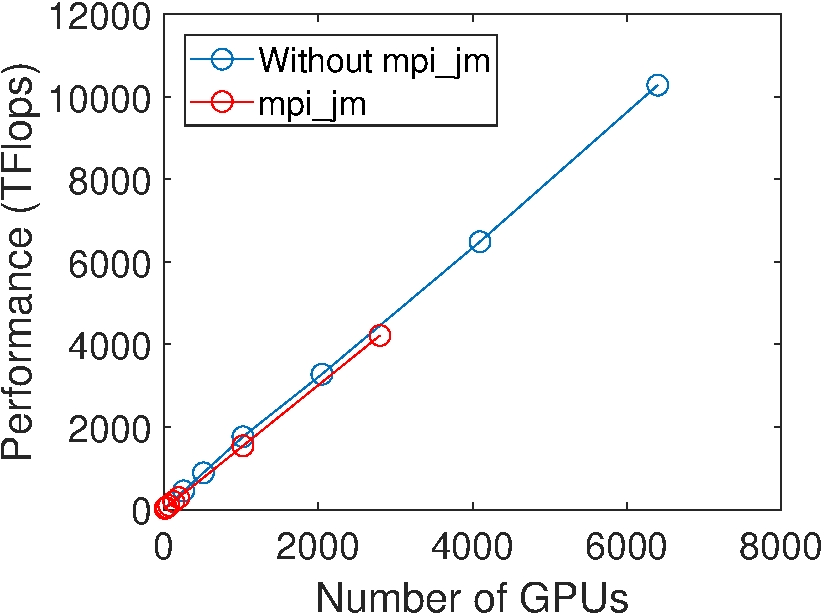
\includegraphics[width=0.6\textwidth]{strong-weak_scale_sierra}
    \caption{Sustained performance as one scales GPU-hungry lattice QCD tasks with the available allocation.}
    \label{fig:sierra}
\end{figure}

We encountered unexpected problems when launching on a very large number of nodes (\mpirun encountered some limitations that we now known can be cured with particular command-line arguments).
However, up to that limit, we found identical scaling with just the naively-expected scaling.
The performance corresponds to a sustained $\sim20\%$ of peak possible performance, and we expect to be able to scale to arbitrary allocation size while still relying on only a single invocation of \mpirun (or equivalent).

